%%%%%%%%%%%%%%%%%%%%%%%%%%%%%%%%%%%%%%%%%
% Beamer Presentation
% LaTeX Template
% Version 1.0 (10/11/12)
%
% This template has been downloaded from:
% http://www.LaTeXTemplates.com
%
% License:
% CC BY-NC-SA 3.0 (http://creativecommons.org/licenses/by-nc-sa/3.0/)
%
% Modified by Jeremie Gillet in November 2015 to make an OIST Skill Pill template
%
%%%%%%%%%%%%%%%%%%%%%%%%%%%%%%%%%%%%%%%%%

%----------------------------------------------------------------------------------------
%	PACKAGES AND THEMES
%----------------------------------------------------------------------------------------

\documentclass{beamer}

\mode<presentation> {

\usetheme{}

\definecolor{OISTcolor}{rgb}{0.65,0.16,0.16}
\usecolortheme[named=OISTcolor]{structure}

%\setbeamertemplate{footline} % To remove the footer line in all slides uncomment this line
%\setbeamertemplate{footline}[page number] % To replace the footer line in all slides with a simple slide count uncomment this line

\setbeamertemplate{navigation symbols}{} % To remove the navigation symbols from the bottom of all slides uncomment this line
}

% Setting frametitle to be std
\setbeamercolor{frametitle}{bg=white, fg=black}
\setbeamertemplate{frametitle}[default][center]

%\usepackage{CJKutf8}
%\newcommand{\cntext}[1]{\begin{CJK}{UTF8}{gbsn}#1\end{CJK}}
\usepackage{amsmath,amsthm, amssymb, latexsym, mathptmx, mathtools}
\usepackage{graphicx} % Allows including images
%\usepackage{booktabs} % Allows the use of \toprule, \midrule and \bottomrule in tables
\usepackage{textpos} % Use for positioning the Skill Pill logo

% For code displays
\usepackage{listings}
\usepackage{color}
\usepackage{braket}
\usepackage{multimedia}

\setbeamertemplate{itemize items}[default]
\setbeamertemplate{enumerate items}[default]

\definecolor{dkgreen}{rgb}{0,0.6,0}
\definecolor{gray}{rgb}{0.5,0.5,0.5}
\definecolor{mauve}{rgb}{0.58,0,0.82}

\lstset{frame=tb,
  language=python,
  aboveskip=3mm,
  belowskip=3mm,
  showstringspaces=false,
  columns=flexible,
  basicstyle={\small\ttfamily},
  numbers=none,
  numberstyle=\tiny\color{gray},
  keywordstyle=\color{blue},
  commentstyle=\color{dkgreen},
  stringstyle=\color{mauve},
  breaklines=true,
  breakatwhitespace=true,
  tabsize=3
}



%----------------------------------------------------------------------------------------
%	TITLE PAGE
%----------------------------------------------------------------------------------------

\title[Presentation Skills]{Intro to GPU Computing} 
\author{\textbf{J. Schloss}} % Your name
\institute[OIST] % Your institution as it will appear on the bottom of every slide, may be shorthand to save space
{
Okinawa Institute of Science and Technology Graduate University\\ % Your institution for the title page
Quantum Systems Unit\\
\textit{james.schloss@oist.jp} % Your email address
}
\date{\today} % Date, can be changed to a custom date

\begin{document}

\usebackgroundtemplate{%
  
\includegraphics[width=\paperwidth,height=\paperheight]{OISTBG}} 
\begin{frame}
\centering
    \titlepage % Print the title page as the first slide
\end{frame}

\usebackgroundtemplate{
    
\includegraphics[width=\paperwidth,height=\paperheight]{PPTBG}}

\setbeamertemplate{background}{} % No background logo after title frame

\begin{frame}
\frametitle{Why use GPU computing?}

General Purpose Graphical Processing Unit (GPGPU) computing is a great step towards HPC computing on consumer hardware. It works best with programs that are:
\begin{itemize}
\item Data parallel (can act independently on different elements)
\item Throughput intensive (There are a lot of elements)
\end{itemize}

\begin{figure}
\begin{center}
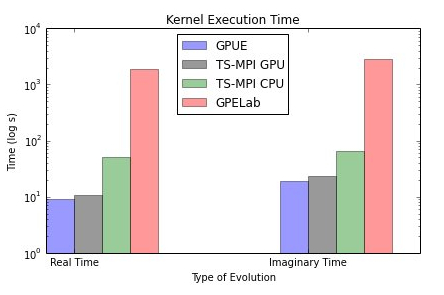
\includegraphics[width=0.4\textwidth]{GPUE_BENCHMARKS.jpg}
\end{center}
\caption{\url{http://peterwittek.com/gpe-comparison.html}}
\end{figure}
\end{frame}

\begin{frame}
\frametitle{GPU vs CPU}
GPU Computing can do many things much faster than the CPU; however, there are a few drawbacks:
\begin{center}
\begin{tabular}{c | c | c}
& CPU & GPU \\
\hline
Memory & 128GB & ~12GB \\
& & \\
Parallelization & afterthought & natural \\
& OpenMP, MPI & CUDA, OpenCL...\\
Boilerplate & a little & a lot\\

\end{tabular}
\end{center}
\end{frame}

\begin{frame}
\frametitle{Parallelization}
\begin{columns}
\column{0.5\textwidth}
In most GPU simulations, data is parsed into \textbf{threads}(work-item), \textbf{blocks}(work-group), and a \textbf{grid}(NDRange).
\begin{itemize}
\item Threads have fast \textit{shared memory} within a block.
\item Data parallelism within a block
\end{itemize} 
\column{0.5\textwidth}
\begin{center}
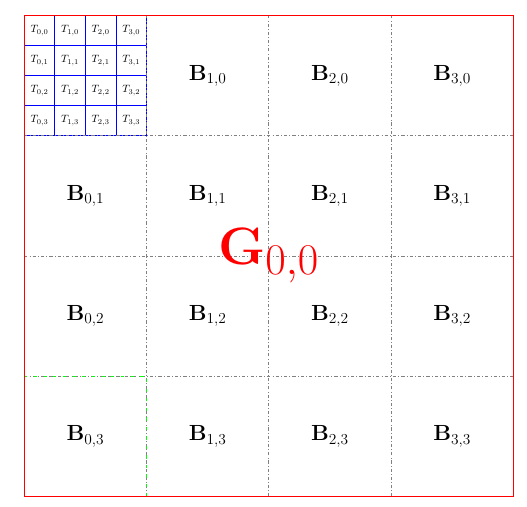
\includegraphics[width=\textwidth]{GBT.png}
\end{center}
\end{columns}
\end{frame}

\begin{frame}
\frametitle{Hardware}
There are two major vendors for GPU's: 
\begin{description}
\item[AMD] ``Open'' computing (Must use \textbf{OpenCL})
\item[nVidia] ``Industry standard'' for GPU computing (can use \textbf{OpenCL} or \textbf{CUDA}). 
\end{description}

For the most part, these follow trends you hear about in gaming: nVidia trail-blazes and AMD keeps up; however, this is not necessarily true with recent cards.

\vspace{0.5cm}

OpenCL and CUDA are comparable in performance, though CUDA has more robust libraries.
\end{frame}

\begin{frame}
\frametitle{CUDA}
\vspace{-0.5cm}

CUDA (once Compute Unified Device Architecture) is the standard programming language to use for GPGPU computing and boasts speed and performance; however, it only works on nVidia cards.

\vspace{0.5cm}
In GPU computing, functions are called \texttt{kernels}:
\begin{description}
\item [\texttt{\_\_global\_\_}] May be called from the host or device
\item [\texttt{\_\_device\_\_}] Must be called from the device
\item [\texttt{\_\_host\_\_}] Is just a normal function
\end{description}

There are also a bunch of CUDA-specific functions(\texttt{cudaMalloc}, \texttt{cudaMemcpy}, \texttt{cudaFree}, etc...)

\vspace{0.5cm}
A quick example of vector addition can be found in the git repo under \texttt{intro/CUDA}

\end{frame}

\begin{frame}
\frametitle{CUDAnative.jl}
This is a julia implementation of CUDA and will be developed further in the future. 

\begin{itemize}
\item It is much easier to use than CUDA and works well with most Julia code.
\item It is incomplete and hard to build
\item More informationa can be found here: \url{http://juliagpu.github.io/CUDAnative.jl/stable/man/usage.html}
\end{itemize}

\end{frame}

\begin{frame}
\frametitle{OpenCL}

OpenCL is the Open Computing Language created by Khronos (OpenGL, Vulkan) and...

\begin{itemize}
\item Follows similar notation to OpenGL. In OpenGL, shaders are read in as strings, but in OpenCL, kernels are read in as strings
\item Allows users to use all hardware on their computer in the same language, including CPU, GPU, FPGA, etc...
\item Also allows for OpenGL interoperability for visualizations
\end{itemize}

A quick example of vector addition can be found in the git repo under \texttt{intro/OpenCL}
\end{frame}

\begin{frame}[fragile]
\frametitle{Accessing GPU's at OIST}

After logging on to Sango or Tombo, you can check which GPU's are taken with 

\begin{lstlisting}
squeue -p gpu
\end{lstlisting}

and can access a GPU node (interactively) with

\begin{lstlisting}
srun --partition=gpu --gres=gpu:1 --pty /bin/bash
\end{lstlisting}

Once you have access, you can check each GPU with \texttt{nvidia-smi}
\end{frame}

\end{document} 
